\ifx \globalmark \undefined %% This is default.
	\documentclass[twoside,openright,11pt,a4paper]{report}

%\compiler avec xelatex
%\usepackage[applemac]{inputenc}
\usepackage[T1]{fontenc}
\usepackage[utf8]{inputenc} %latin1 est possible
%\usepackage[latin1]{inputenc} %latin1 est possible
\usepackage[UKenglish]{babel}
\usepackage{lettrine}

%\usepackage[text={13cm,20cm},centering]{geometry}
\usepackage [squaren, Gray, mediumqspace]{SIunits}
\usepackage [top=2cm, bottom=2cm, left=2cm, right=2cm ]{geometry}

\renewcommand{\familydefault}{cmss}
\addto\captionsenglish{ \renewcommand\chaptername{Solutions of Chapte}}

\usepackage{graphicx}
\usepackage{amsmath}
\usepackage{amsfonts}
\usepackage{amssymb}
\usepackage{amsthm}
\usepackage{bm}
\usepackage{color}

\newcommand{\real}{\mathbb{R}}
\newcommand{\mb}{\mathbf}
\newcommand{\bos}{\boldsymbol}

\def \RR {I \! \! R}

\newcommand{\e}{\begin{equation}}  
\newcommand{\ee}{\end{equation}}
\newcommand{\eqn}{\begin{eqnarray}} 
\newcommand{\eeqn}{\end{eqnarray}} 
\newcommand{\eqnn}{\begin{eqnarray*}} 
\newcommand{\eeqnn}{\end{eqnarray*}} 

\newcommand{\bpm}{\begin{pmatrix}}
\newcommand{\epm}{\end{pmatrix}}

%\newcommand{\{\c c}}{\c c}

\newcommand{\bma}{\left(\begin{array}}
\newcommand{\ema}{\end{array}\right)} 
\newcommand{\hh}{\hspace{2mm}}
\newcommand{\hd}{\hspace{5mm}}
\newcommand{\hu}{\hspace{1cm}}
\newcommand{\vv}{\vspace{2mm}}
\newcommand{\vd}{\vspace{5mm}}
\newcommand{\vm}{\vspace{-2mm}}
\newcommand{\teq}{\triangleq}
%\newcommand{\qedb}{\,$\Box$}
\newcommand{\blanc}{$\left. \right.$}
\newcommand{\frts}[2]%
         {\frac{{\textstyle #1}}{{\textstyle #2}}}

\newcommand{\bindex}[3]%
{
\renewcommand{\arraystretch}{0.5}
\begin{array}[t]{c}
#1\\
{\scriptstyle #2}\\
{\scriptstyle #3}
\end{array}
\renewcommand{\arraystretch}{1}
}

\theoremstyle{definition}
\newtheorem{exemple}{{\bf Exemple}}[chapter]
\newtheorem{theoreme}[exemple]{{\bf Th{é}or{è}me}}
\newtheorem{propriete}[exemple]{{\bf Propri{é}t{é}}}
\newtheorem{definition}[exemple]{{\bf D{é}finition}}
\newtheorem{remarque}[exemple]{{\bf Remarque}}
\newtheorem{remarques}[exemple]{{\bf Remarques}}
\newtheorem{lemme}[exemple]{{\bf Lemme}}
\newtheorem{hypothese}[exemple]{{\bf Hypoth{è}se}}
\newtheorem{exercice}{{\bf Exercice}}[chapter]

\newcommand{\xqedhere}[2]{%
 \rlap{\hbox to#1{\hfil\llap{\ensuremath{#2}}}}}

\newcommand{\xqed}[1]{%
 \leavevmode\unskip\penalty9999 \hbox{}\nobreak\hfill
 \quad\hbox{\ensuremath{#1}}}

\newcommand{\gf}{\fg\,\,}

\newcommand{\cata}[1] %
     {\renewcommand{\arraystretch}{0.5}
     \begin{array}[t]{c} \longrightarrow \\ {#1} \end{array}
     \renewcommand{\arraystretch}{1}}

\usepackage[isu]{caption}
%\usepackage[font=small,format=plain,labelfont=bf,up,textfont=it,up]{caption}
\setlength{\captionmargin}{60pt}

\newcommand{\cqfd}
{%
\mbox{}%
\nolinebreak%
\hfill%
\rule{2mm}{2mm}%
\medbreak%
\par%
}

\pagestyle{headings}

\renewcommand{\sectionmark}[1]{%
\markright{\thesection.\ #1}{}}

\renewcommand{\chaptermark}[1]{%
\markboth{\chaptername\ \thechapter.\ #1}{}}

\makeatletter 
\def\@seccntformat#1{\csname the#1\endcsname.\;} 
\makeatother

\title{ {\Huge {\textbf{Modélisation et analyse  \\ \vspace{4mm} des systèmes dynamiques }}} \\ \vspace{4cm} G. Bastin}

%\title{ {\Huge {\textbf{Modelisation et analyse  \\ \vspace{4mm} des systemes dynamiques }}} \\ \vspace{4cm} G. Bastin}


\date{\today}
	\begin{document} %% Crashes if put after (one of the many mysteries of LaTeX?).
\else 
	\documentclass{standalone}
	\begin{document}
\fi

\graphicspath{ {Chapitre1/images/} }

\setcounter{chapter}{0}
\chapter{Dynamic systems and state models}
\chaptermark{Dynamic systems and state models}


\lettrine[lines=1]{\bf I}{}n this first chapter we give first of all the definition of the dynamic systems group which is studied in the book, as well as the terminology and the used notations, and we illustrate it with some examples from engineering sciences. We explain then what recover the notions of modelling and analysis of dynamic systems. The chapter ends by a brief description of the nine other chapters content.

\section{Definitions and examples} \label{exemple}

In this book, we will study dynamic systems described by sets of first-order differential equations of the shape
\eqn
\dot x_1&=&f_1(x_1,x_2, \ldots, x_n,u_1,u_2, \ldots u_m), \nonumber\\
\dot x_2&=& f_2(x_1,x_2, \ldots, x_n,u_1,u_2, \ldots u_m), \nonumber\\
\vdots&&\vdots\label{eq:modetn}\\
\dot x_n &=& f_n(x_1,x_2, \ldots, x_n,u_1,u_2, \ldots u_m), \nonumber
\eeqn
where $f_i$ are applications from $\real^{n+m}$ to $\real$, while the $x_i$ and $u_i$ are scalar functions of {\em time} $t$, which is an independant variable. The quantity $\dot x_i$ represents the derivative of the variable $x_i$ relative to time $t$.  The variables $x_1, x_2, \ldots, x_n$ are called {\em state variables} and contain all the necessary information on {\em the state} of the system in the present to be able to measure its evolution in the future, by means of equations (\ref{eq:modetn}), knowing the future values of the variables $u_1, u_2, \ldots, u_m$. 
These are called {\em entries} of the system, and represent the outside's influence on the studied system.  We often write, in a condensed way, 
\e
\dot x = f(x,u)\label{eq:modet}
\ee
where $f$ is an application from $\real^{n+m}$ to $\real^n$ while $x$ and $u$ are vectorial functions of time. 

Such a system of
equations is called {\em state model}. The goal of this book is to treat the {\em modelling},  i.e. obtaining such equations for diverse applications of engineering sciences, and the {\em analysis}, i.e. the determination of
main properties of these systems, deducted from the equations. 
Let us begin with some examples to illustrate our subject.
\vv

\begin{exemple}{\bf A glass furnace}

The first example is an industrial process, illustrated in figure \ref{fig:fourverre}.  
\begin{figure}[t]
\begin{center}
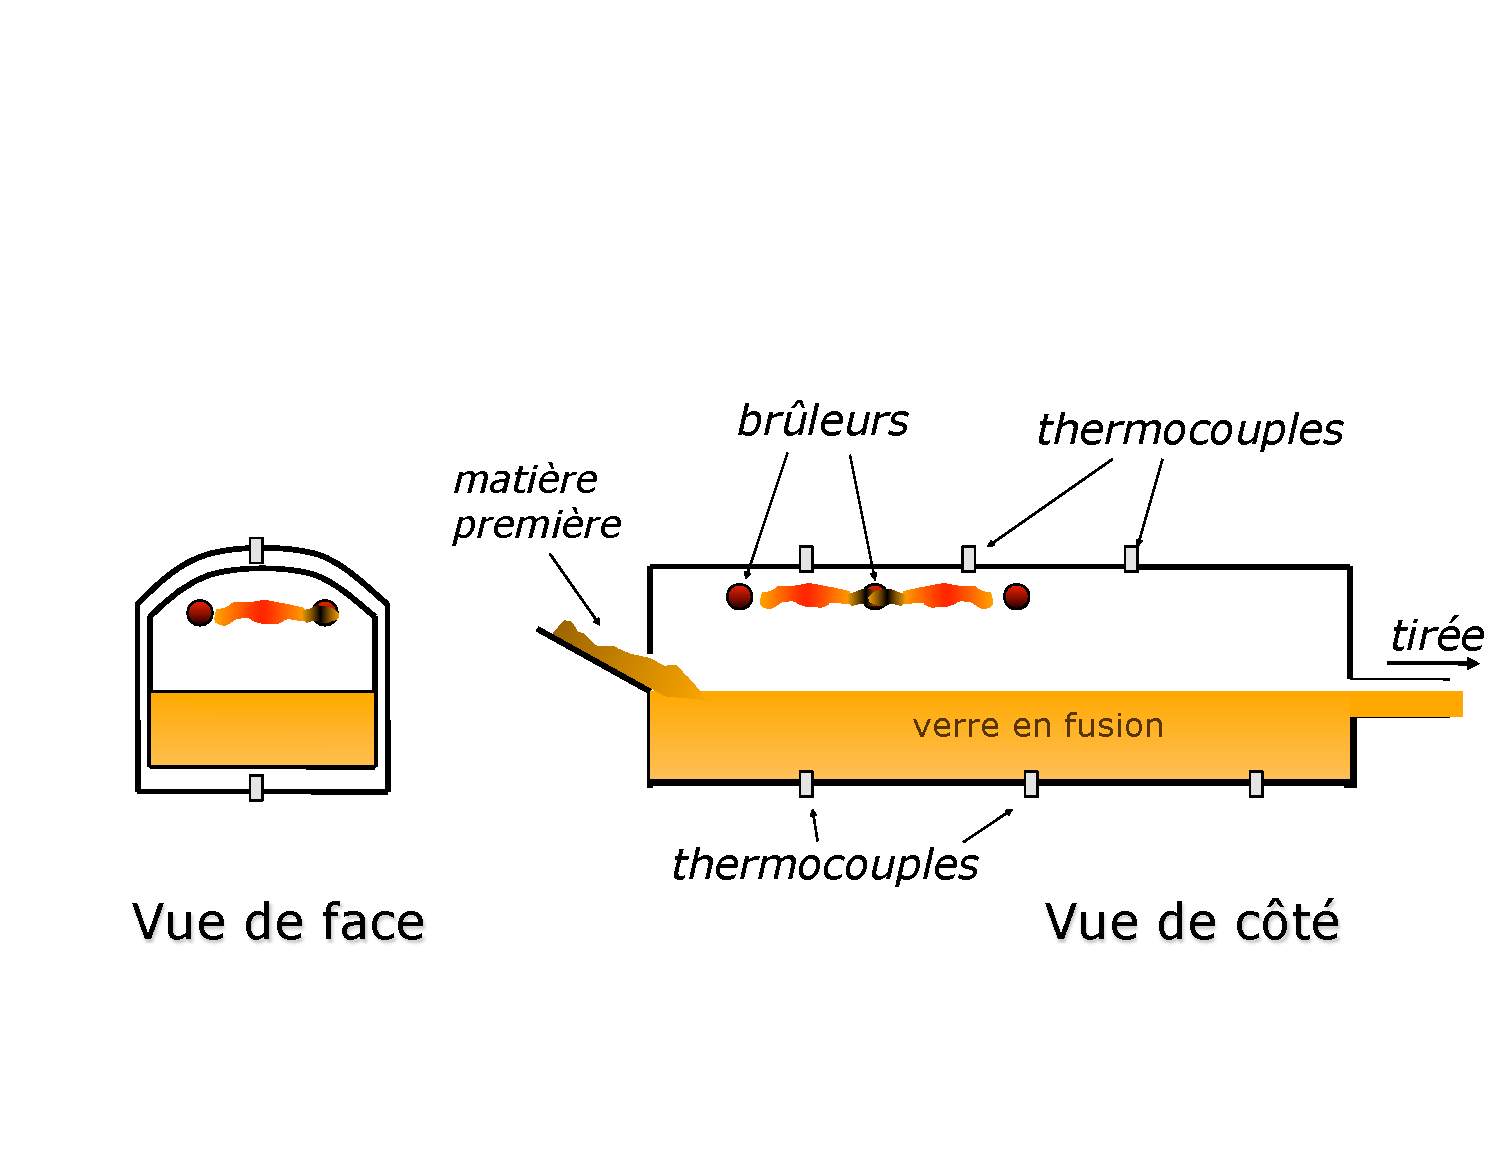
\includegraphics[width=12cm]{fouraverre}
\caption{A glass furnace}
\label{fig:fourverre}
\end{center}
\end{figure}
It is about a furnace whose walls are built in refractory material and in which we melt a mixture
of sand, lime and other additives to obtain glass. This fusion is
obtained thanks to an energy input inside the furnace, for
instance coming from a gas burner placed above the bath of
glass. The molten glass is extracted from the furnace in a continuous way
to feed machines downstream. By making the assumption that the temperature of the glass is homogeneous in
the furnace and that this one is perfectly isolated, we can write the
following equations, corresponding to the mass balance and to the energy balance of
the process. We thus write that the mass or energy change in the considered system, by unit of time, equals the
sum of what goes into the system, in terms of mass and heat,
decreased by what gets out of it, always during the same unit of time:
\eqn \begin{split}
\frac{dM}{dt} &= P_{in} - P_{out}, \label{eq:bvf} \\
\frac{d}{dt}(CTM) &= Q_{in} + C_{in}T_{in}P_{in}-CTP_{out},
\end{split} \eeqn
with the following meaning of variables and parameters of the model:\\

$M$ : mass of the glass in fusion in the furnace (kg),

$T$ : temperature of the glass in fusion in the furnace (K),

$T_{in}$ : temperature of the row material put in the furnace (K),

$C$ : specific heat of the glass (J/K$\times$kg),

$C_{in}$: specific heat of the raw material (J/K$\times$kg),

$Q_{in}$ : heat quantity supplied by unit of time (J/s),

$P_{in}$ : mass put in the furnace by unit of time (kg/s),

$P_{out}$ : mass extracted by unit of time (kg/s).\\

\noindent We indicated units for each of the sizes defined above. The dimensional coherence of the equations is the first check to be made in an exercise of transforming a mathematical model into equations.

In order to put the system of equations (\ref {eq:bvf}) under the shape of a state model (\ref {eq:modetn}), we define the state variables ~: \\

$x_1 \triangleq M$ : mass of the glass in fusion (kg),

$x_2 \triangleq C T$ : heat quantity by unit of mass of glass in fusion (J/kg),\\

\noindent and the input variables~:\\

$u_1 \triangleq P_{in}$ : mass put in the furnace by unit of time (kg/s),

$u_2 \triangleq P_{out}$ : mass extracted by unit of time (kg/s),

$u_3 \triangleq Q_{in}$ : head supplied by unit of time (J/s).\\

\noindent We obtain the following state model~:
\begin{equation} \begin{split} \label{four1}
\dot x_1 &= u_1 - u_2, \\
\dot x_2 &= \dfrac {u_1(\alpha - x_2) + u_3}{x_1},
\end{split} \end{equation}
where the constant parameter $\alpha = C_{in}T_{in}$ is the heat quantity of the material put in the furnace by unit of mass.

Note that other choices for the state variables and input variables are possible (see exercise 1.2). \qed
\end{exemple}  
\vv

\begin{exemple}{\bf  A chemical reactor }

\begin{figure}[ht]
\begin{center}
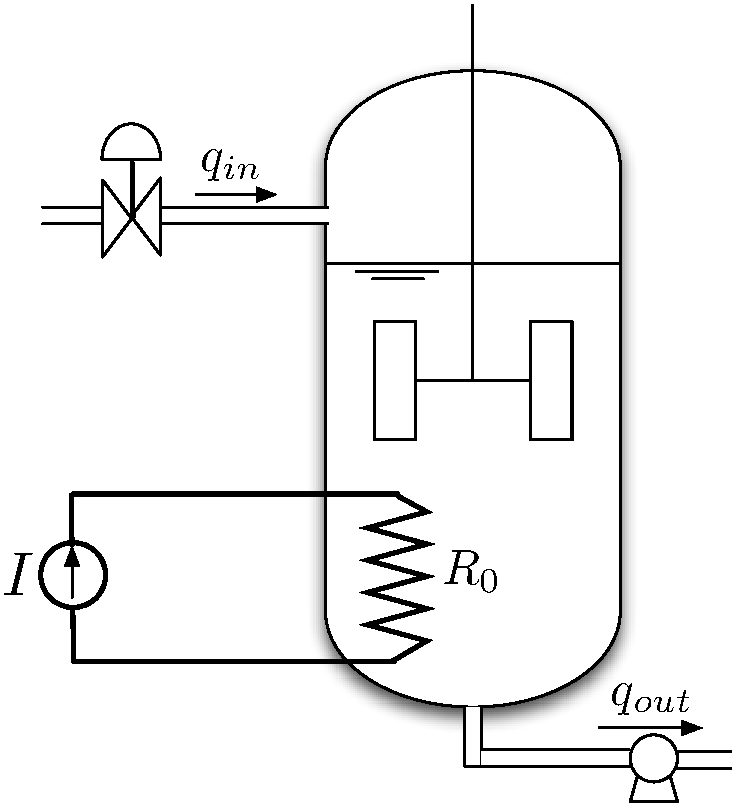
\includegraphics[width=7cm]{reachim}
\caption{Chemical reactor}
\label{fig:reachim}
\end{center}
\end{figure}
In a chemical reactor (Figure \ref{fig:reachim}), a reaction transforming a reactive A into a product B takes place in liquid phase with a certain temperature  $T$.  The reactor is fed with reactive
A via a valve wich introduces the reactive with concentration
$A_{in}$ with a variable volume flow
$q_{in}$ which is a monotonous increasing function of the valve opening $w$ : $q_{in} = \phi(w)$. The content of the reactor is extracted by a pump with a flow $q_{out}$. We assume that the reaction is endothermic and then requires a heat input $W$ supplied by a heating resistance $R_0$ fed by a variable current source $I$ as illustrated in the figure. Moreover, we assume that the reactor is
perfectly mixed. The reaction (i.e. the transformation of the reactive A in
produced B) takes place with a reaction speed which follows a kinetic of the first order, i.e. proportional to the quantity of reactive A in the
reactor. The coefficient of proportionality is a function of the temperature
and verify the law of Arrhenius, $k(T)=k_0 \exp(-\frac{E}{RT})$.\\

We describe the evolution of this system by writing the equations of volumetric, mass and heat balances:
\begin{equation*} \begin{split} 
&\frac{dV}{dt} = q_{in} - q_{out},\\[0.3em]
&\frac{d}{dt}(AV) = q_{in}A_{in} -q_{out}A-k(T)AV, \\[0.3em]
&\frac{d}{dt}(BV) = -q_{out}B + k(T)AV, \\[0.3em]
&\frac{d}{dt}(CTV) = CT_{in}q_{in}-CTq_{out} - hk(T)AV + R_0I^2,
\end{split} \end{equation*}
with~:\\

$V$ : liquid volume in the reactor, 

$A$ : concentration of reactive A in the reactor,

$B$ : concentration of reactive B in the reactor,

$k_0$ : reaction speed's constant,

$E$ : activation energy,

$R$ : Boltzmann constant,

$C$ : specific heat,

$h$ : reaction enthalpy.\\

\noindent The other notations are defined above. We can define the state variables

$x_1 = A$ : reactive concentration in the reactor,

$x_2 = B$ : product concentration in the reactor,

$x_3 = V$ : volume of the reactionnal environment,

$x_4 = T$ : temperature of the reactionnal environment,\\

\noindent and the input variables

$u_1 = w$ : valve opening,

$u_2 = q_{out}$ : withdrawal rate,

$u_3 = I$ : electrical current supplied in the heating resistance,\\

\noindent we obtain the following state model~:
\begin{equation*} \begin{split} 
\dot x_1 &= \phi(u_1)\dfrac{{\textstyle A_{in} - x_1}}{{\textstyle x_3}} - k(x_4)x_1,\\[0.3em]
\dot x_2 &= - \phi(u_1) \dfrac{x_2}{x_3} + k(x_4)x_1,\\[0.3em]
\dot x_3 &= \phi(u_1) - u_2, \\[0.3em]
\dot x_4 &= \dfrac{{1}}{{x_3}}[\phi(u_1)(T_{in} - x_4) + \dfrac{{R_0}}{{C}}u_3^2] - \dfrac{{h}}{{C}}k(x_4)x_1.
\end{split} \end{equation*}
{\it Continuous} and {\it isotherms} reactors constitute an interesting particular case. It is about reactors for which the volume $V$ and the temperature $T$ are maintained constant by adequate regulation devices. The state model is then reduced to the first two equations of the model above ~:
\begin{equation} \begin{split} \label{iso}
\dot x_1 &= \dfrac{\phi(u_1)}{{V}} (A_{in} - x_1) - k(T)x_1, \\[0.3em]
\dot x_2 &= - \dfrac{\phi(u_1)}{{V}} x_2 + k(T)x_1.  \xqedhere{4.8cm}{\qed}
\end{split} \end{equation}
\end{exemple}
\vv

\begin{exemple}{\bf Ladybirds and aphids}

Aphids are permanent pests for the rosebushes cultures. The biological fight against these devastating species is an alternative to the treatments by pesticides, which are less and less effective in front of the resistances developed by aphids.
\begin{figure}[ht]
\begin{center}
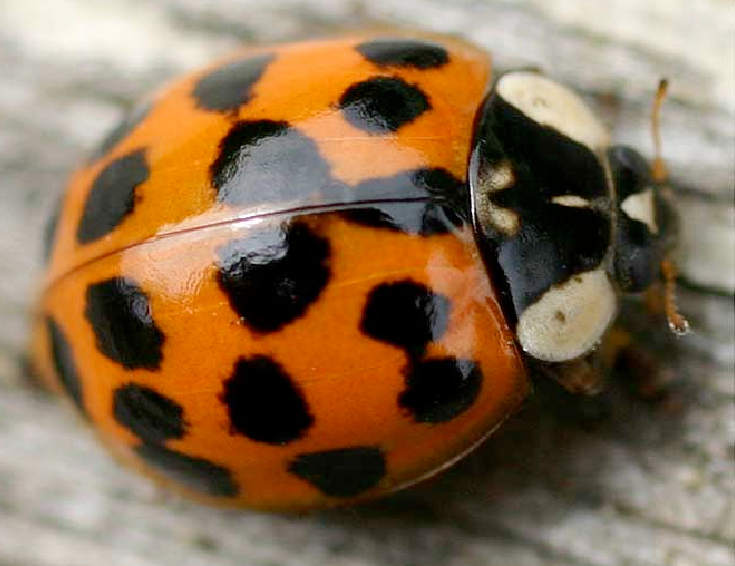
\includegraphics[width=4cm]{cocci}
\caption{Harmonia axyridis}
\label{fig:cocci}
\end{center}
\end{figure}
The {\em Harmonia axyridis} ladybirds (Fig. \ref{fig:cocci}) are used in this biological fight because they feed on aphids with great voracity. They are active by spring, that is by the appearance of the aphids colonies in rose gardens. To increase the predatory efficiency of ladybirds, the French institute of agronomic research (INRA) developed a ladybirds variety \og home-bodies \gf who do not fly (and therefore are not likely to leave the cultures).

We wish to establish a model describing the evolution of the number of aphids $x_1(t)$ and of ladybirds $x_2(t)$ under the following assumptions:
\begin{enumerate}
\item if there are no ladybirds, the population of aphids has enough food (rosebushes leaves) to have an exponential growth with a specific constant rate of growth;
\item ladybirds eat more aphids if their population is bigger;
\item the predation by ladybirds is the only source of aphids natural mortality;
\item ladybirds have a constant specific rate of natural mortality;
\item the gardener, who is not very smart, spreads a pesticide which kills indifferently aphids and ladybirds with a variable manuring rate  $u(t)$.
\end{enumerate}
The following state model expresses the balance of the number of aphids and ladybirds:
\begin{equation} \begin{split}  \label{coc}
\dot x_1 &= ax_1 - bx_1x_2 - cux_1, \\
\dot x_2 &= dx_1x_2 - ex_2 - fux_2. 
\end{split} \end{equation} 
where $a,b,c,d,e,f$ are positive constants. We can verify that every term of this model formalizes one of the assumptions above. This check is left as exercise.\\

This type of model was originally introduced by the Italian mathematician V. Volterra who tried to understand the fluctuations in the efficiency of the fishing in Adriatic sea at the beginning of the twentieth century. Obviously, it is a rather big simplification of the reality. The model doesn't take into account numerous factors that can influence the evolution of the populations (weather conditions, other available resources, other predators, migration of the populations etc.). As our example shows it, an important application of this type of model is the fight against pests in the agriculture. It often happens that the harmful population is controlled by predator introductions. The model is then an interesting tool for the design of intervention programs on the ground. \qed \\
\end{exemple}


\begin{exemple}{\bf A DC motor}

We now examine the electromechanical device shown in figure \ref{fig:motdc}.
\begin{figure}[ht]
\begin{center}
\includegraphics[width=6cm]{motdc}
\caption{DC motor}
\label{fig:motdc}
\end{center}
\end{figure}
This is a DC motor which can be controlled by both the stator voltage $e$ and the rotor current $I$.
The stator circuit equation is given by
\eqnn
e=Ri+L\frac{di}{dt}
\eeqnn
where $R$ and $L$ are the resistance and inductance of the circuit,
$e$ is the control voltage and $ i$ is the current. The couple
exerted on the rotor is given by $C = \Phi I$ where $I$ is the rotor current and $\Phi$ is the magnetic flow
proportional to the excitation current $\Phi = Ki$. We therefore obtain
\eqnn
C=KiI.
\eeqnn
It remains to model the mechanical part of the system. Noting $\theta$ the
angular position of the rotor, $J$ its moment of inertia and $F$ the viscous friction coefficient, the application of Newton's law leads to~:
\eqnn
J\frac{d^2\theta}{dt^2}+F\frac{d\theta}{dt}=C.
\eeqnn

We can define the state variables $x_1=\theta, x_2=\dot{\theta}, x_3=i$, the inputs $u_1=e$, $u_2=I$, and we obtain the following state model:
\begin{equation} \begin{split} \label{motDC}
\dot x_1 &= x_2,  \\[0.3em]
\dot x_2 &= -\frac{F}{J}x_2+\frac{K}{J}x_3u_2, \\[0.3em]
\dot x_3 &= -\frac{R}{L}x_3+\frac{1}{L}u_1. \xqedhere{5cm}{\qed}
\end{split} \end{equation}
\end{exemple}
The four examples we just discussed are intended to show
that equation (\ref{eq:modet}) actually helps to build models of dynamic systems in various application areas
of engineering as we treated successively examples about thermodynamics, chemical engineering, ecology and electronics. They will also help to understand better the terminology that is introduced in the next section. 

\section{Terminology and notations}

As the previous examples illustrated it, we study {\em dynamic systems} whose behavior is described by a {\em state model} composed by a set of differential equations written under condensed shape:
\eqn
\dot x = f (x, u). \label{sysdyn}
\eeqn
We consider this state model from an initial time $t_0$. 
The state $x \in \real^n$ and the entry $u \in \real^m$ are vectorial functions of
time that we can sometimes note $x(t)$ and $u(t)$. However,
the argument $t$ is often omitted without confusion.

For a given system, the entry $u(t)$ is a priori any function of the time. However, we always assume that it is a {\em piecewise continuous} and {\em bounded} function ~: $u(t) \in {\cal U}$ where ${\cal U}$ is a set of piecewise continuous and
bounded of $\real$ to $\real^m$ functions.

For a given value of the initial state $x(t_0) = x_0$ and an input $u(t)$ given, the solution $x(t) \;\; t \geq t_0$ of the differential system
(\ref{sysdyn}) is called {\em path} of the system. Sometimes, when it
will be necessary for the presentation clarity, the path will be denoted
$x(t, x_0, u)$. We always assume that such a path exists
at any time $t \geq t_0$, is unique and is a continuous function of time.
Graphically, a path may be displayed by a continuous curve in $\real^{n+1}$. The path projection in the
{\em state space} $\real^n$ (also called {\em phase space}) is called
an {\em orbit} of the system.

When the input $u(t)$ can be freely chosen in ${\cal U}$, we say
that the system $\dot x = f(x,u)$ is a {\em forced} system, or a {\em controlled} system. The term {\em forced} is used to
mean that starting from an initial state $x_0$, the shape of the path
is somehow forced by the choices we made of an input $u(t)$. Similarly, in an automatic context, the term {\em controlled}
means that the system state can be manipulated in the state space by suitable manipulation of the input $u(t)$.

In the next chapters however, we will be interested in the solution of the equation $\dot x = f(x,u)$ when the input is
actually a constant fixed a priori : $u(t) = \bar u \;\; \forall t \geq
t_0$.  In that case, we write the state model as $\dot x = f(x,
\bar u)$.  We sometimes also write 
\eqnn
\dot x = f_{\bar u} (x)
\eeqnn
to express more clearly that $f$ is only a function of $x$,
parameterized by the constant $\bar u$. In such a case, there is
only one possible path moving freely at the start of an initial state  $x_0$. By fixing in advance the input at a constant value, we have no longer the ability to control the paths of the system and say that
the system is a {\em free} system (we also say an {\em autonomous} system, or
{\em stationary} system). The path is sometimes called {free response} of the system.

When we are interested in the solution of the equation $\dot x = f(x,u)$ for
{\em one} input $u(t)$ that is not constant over time but specific (for
example a sine wave), we may as well forget that we
selected an input in ${\cal U}$ and simply write:
\eqnn
\dot x = f(x,t)
\eeqnn
A dynamic system represented this way is called a {\em  non-autonomous} or {\em unstationary} system. 

We will sometimes consider various special cases of the
general state model (\ref{sysdyn}). We distinguish in particular~;\\

\noindent \textbf{\textit{Affine systems relative to the input}}
\eqnn
\dot x = f(x) + \sum^m_{i=1} u_ig_i(x) \triangleq f(x) + G(x)u
\eeqnn
where $f$ and the $g_i$ are applications from $\real^n$ to $\real^n$.
The state model \eqref{four1} of a glass furnace is of this form with the following definitions~:
\begin{equation*}
f(x) = 0, \hh \hh \hh \hh G(x) = \left(\begin{array}{ccc}
1&-1 & 0 \\[0.3em] (\alpha-x_2)/x_1 & 0 & 1/x_1 \end{array} \right).
\end{equation*}\\

\noindent \textbf{\textit{ffine systems relative to the state}}
\eqnn
\dot x = \sum^m_{i=1}x_i a_i(u) + b(u) \triangleq A(u) x + b(u) 
\eeqnn
where $b$ and the $a_i$ are applications from $\real^m$ to $\real^n$. The state model of an isothermal continuous chemical reactor \eqref{iso} is of this form with the following definitions~:
\begin{equation*} \begin{split}
A(u) &= \left(\begin{array}{cc}
-(\dfrac{\phi(u_1)}{V} +k(T)) & 0 \\[0.3em] k(T) & -\dfrac{ \phi(u_1)}{V}
\end{array} \right),\\[0.5em]
b(u) &=  \left(\begin{array}{c} \dfrac{ \phi(u_1) A_{in}}{V}\\[0.7em] 0
\end{array}\right).
\end{split} \end{equation*}\\

\noindent \textbf{\textit{The bilinear systems}}
 
These systems are affine relative both to the state and the input
\begin{eqnarray*}
\dot x &=& \left ( A_0 + \sum^m_{i=1} u_iA_i \right) x + B_0u, \\[0.3em]
&=& A_0x + (B_0+ \sum^n_{i=1} x_i B_i)u,
\end{eqnarray*}
where the $A_i$ $(i = 0, \ldots, m)$ are matrices of dimension $(n
\times n)$ and the $B_i$ $(i = 0, \ldots, n)$ are matrices of
dimension $(n \times m)$.  The state model of a DC motor
(\ref{motDC}) is of this form with the following definitions~:
\begin{equation*} \begin{split}
A_0 &= \left( \begin{array}{ccc}
0 & 1 & 0 \\[0.3em] 0 &-\dfrac{B}{J} & 0\\[0.3em]
0&0& -\dfrac{R}{L}
\end{array}
\right)\;\;\; A_1 = 0
\\
A_2 &= \left( \begin{array}{ccc}
0 & 0 & 0 \\[0.3em] 0 & 0 & \dfrac{K}{J} \\[0.5em]
0 & 0 & 0
\end{array}\right)\hspace*{10mm} B_0 = \left(\begin{array}{cc} 0 & 0 \\[0.3em] 0 & 0 \\[0.3em] \dfrac{1}{L}&0
\end{array} \right).
\end{split} \end{equation*}\\

\noindent \textbf{\textit{Linear systems}}
$$
\dot x = Ax +Bu
$$
where $A$ is a matrix of dimension $(n \times n)$ and $B$ is a matrix of dimension $(n \times m)$.  If we consider the state model of the DC motor assuming that the rotor current source is constant ($I$ = constant), we obtain an example of a linear system with
\begin{equation*}
A = \left( \begin{array}{ccc}
0 & 1 & 0 \\[0.3em] 0 &-\dfrac{B}{J} & \dfrac{KI}{J}\\[0.9em]
0&0& -\dfrac{R}{L}
\end{array}
\right)\;\;\; B = \left(\begin{array}{cc} 0 & 0 \\[0.3em] 0 & 0 \\[0.3em] \dfrac{1}{L}&0
\end{array} \right).
\end{equation*}
\vv

\section{Modeling and analysis}

A dynamic system, as we conceive it in this book, is thus a part of the {\it concrete} reality that seems relevant in an engineering problem and that we choose to isolate in thought to describe its behavior in mathematical terms using a model. In particular, we are interested in characterize quantitatively the evolution over time of the {\it state} of the system. For this, we use \blue{deterministic, lumped parameters state models} which consist of ordinary differential equations.

However, other modeling approaches of dynamic systems are possible. For the various examples described in the section \ref{exemple} we could have  build \blue{deterministic, {\it distributed parameters} state models} composed of partial differential equations. This is how, in the example of the glass furnace, we made the hypothesis that the temperature was uniform across the glass bath. This is a simplistic view, but very useful to build simple and effective models for instance in view of the control and optimization of the dynamic behavior of the furnace. However, if this hypothesis is not accepted and we want to study the spatial variations of temperature, we can develop a state model consisting of partial differential equations describing the evolution over time of the temperature and velocity of the fluid fields in the molten glass bath. Neither model is better than the other. They simply are different models obtained for different objectives, usually corresponding to different spatial and temporal scales.

The interaction between the system and the \og outside world \gf is represented by the inputs of the model $u_i(t)$ which are, as we mentioned above, functions of time, real and deterministic. In reality, a given system is often subject to random influences that can be represented by introducing stochastic inputs, i.e. random functions $u_i(t) $ (also called stochastic processes). We then obtain stochastic state models whose state variables are themselves random functions and whose study uses different mathematical techniques than those used in this book.

The state model of a dynamic system is thus a simplified mathematical representation of the behavior of the system. Yet, when it will not affect the clarity of the argumentation, we will often consider these two notions as equivalent in order to simplify the presentation. We will then speak of the dynamic system $\dot x = f(x,u)$, implying that we actually speak of a deterministic state model of the system.

The {\it modeling} of a dynamic system, as we conceive it in this book, is thus the exercise that aims to, given a discursive and qualitative description of the system, establish a mathematical description of it as a state model. Without being unnecessarily complicated, the resulting model should be an effective tool for solving the engineering problem posed for the system considered. The assumptions adopted for modeling should be clearly identified and highlighted.

In the first part of the book, we will show
how the modeling approach can be systematized for different
relevant classes of systems in engineering. We will successively discuss mechanical systems, electrical and electromechanical systems,
\blue{compartment systems} and \blue{reaction systems} in Chapters 2-5. In each case, we will 
describe the basic physical principles and how they are
used to obtain the state models. In Chapter 6, we will see how to define and use {\it state transformations} to obtain equivalent models of a given system.

However, we do not intend to describe and justify in detail all the physical principles of the different disciplines which constitute the art of engineering. In more complex modeling cases than those covered in this book, the reader should refer to the literature of the disciplines. However, we hope that the unifying character of the state model concept in engineering sciences will be clearly perceived.

After obtaining the model, we can analyze its properties and derive a certain number of lessons, or on the appropriateness of the model itself, or on the
properties of the dynamic system which is the subject of modeling. It is to this analysis that the second part of the book is dedicated.

In Chapters 7, 8 and 9, we analyze the behavior of dynamic systems which inputs are {\it constant}~: $\dot x= f(x,\bar u)$. In Chapter 7, we first examine the conditions of existence of equilibrium states and invariant subsets of the state space. Chapter 8 is devoted to the study of \blue{{\it plan} systems}, i.e. systems whose state vector is of dimension 2. We examine in particular the behavior of the system near the equilibrium states, as well as periodic trajectories and bifurcations. The purpose of Chapter 9 is to analyze the stability of equilibrium states by the Lyapunov's method and characterize the basins of attraction.

Finally, in Chapter 10, we look at the issue of controllability of dynamical systems that can be formulated as follows: for a forced dynamic system $ \dot x = f(x,u)$, under what conditions and how we can determine the input functions $u_i(t)$ to conduct the system of a given initial $x_0$ state to a given final state $x_f$ in a prescribed time. The answer to this question obviously has important implications in many engineering problems such as \blue{the steering of electro-mechanical devices} or the conduct of industrial processes.
\newpage
\section{Exercices}

\begin{exercice} {\bf \em A glass furnace}

For the glass melting furnace that has been described in this chapter~:
\begin{enumerate}
\item Establish a state model whose state variables are the mass $M$ and the stored heat $C_TM$.
\item Establish a state model whose state variables are the temperature $T$ and the stored heat $C_TM$.
\item Indicate how to change the state model to take into account the heat loss to the outside through the walls of the furnace.
\item The state model was built under the implicit assumption of near-instantaneous fusion of the raw material. Imagine how to easily modify the model to explicitly include the fusion (indication: cut the oven into two compartments of variable mass, one containing the not yet molted material and the other one containing the melt).
\end{enumerate}
\end{exercice}

\begin{exercice}{\bf \em Beetles and aphids}

\begin{enumerate}
\item Justify each term of the model (\ref{coc}) explaining how it formalizes one of the modeling assumptions.
\item Is the model (\ref{coc}) affine in the input, affine in the state, bilinear, linear? 
\item The model (\ref{coc}) was established with two populations : the aphids ($x_1$) and the beetles ($x_2$). The adult beetle can ingest up to 100 aphids per day, but the larvae is even more voracious, it can ingest up to 150 per day. By formulating additional relevant modeling assumptions, establish a more accurate state model distinguishing adult beetles and larvae (i.e. a model with three state variables: aphids ($x_1$), larvae ($x_2$) and adult beetles ($x_3$)).
\end{enumerate}
\end{exercice}



\end{document}
